% !TeX program = pdflatex
\documentclass[11pt,a4paper]{article}
\usepackage[utf8]{inputenc}
\usepackage[T1]{fontenc}
\usepackage{lmodern}
\usepackage{microtype}
\usepackage[main=turkish, english]{babel}
\usepackage{geometry}
\geometry{margin=2cm}
\usepackage{graphicx}
\usepackage{booktabs}
\usepackage{siunitx}
\usepackage{pgfplotstable}
\usepackage[unicode]{hyperref}
\PassOptionsToPackage{hyphens}{url}
\hypersetup{
  colorlinks=true,
  linkcolor=black,
  citecolor=black,
  urlcolor=blue,
  pdftitle={IzmirWildfire2025: Sentinel-2 ile NDVI/NBR Tabanlı Yangın Etki Analizi},
  pdfauthor={Yusuf Talha ARABACI}
}
\usepackage{caption}
\usepackage{subcaption}
\usepackage{amsmath}
\usepackage{float} % For [H] placement
\usepackage[section]{placeins} % Keep floats within their sections

\title{IzmirWildfire2025: Sentinel-2 ile NDVI/NBR Tabanlı Yangın Etki Analizi}
\author{Yusuf Talha ARABACI\\Karabük Üniversitesi\\Yüksek Lisans, Yazılım Mühendisliği Öğrencisi}
\date{Tarih: \today}

\begin{document}
\selectlanguage{turkish}
\sloppy
\maketitle
\thispagestyle{empty}

\clearpage
\tableofcontents
\clearpage

% Turkish abstract (Özet)
\renewcommand{\abstractname}{Özet}
\begin{abstract}
Bu çalışma, 2025 İzmir orman yangınının etkilerini Sentinel-2 L2A verileri kullanılarak
NDVI ve NBR indeksleri üzerinden incelemektedir. Yangın öncesi ve sonrası dönemler için
bulut maskeleme ve median kompozit uygulandıktan sonra NDVI/NBR bantları hesaplanmış,
fark indeksleri (dNDVI, dNBR) türetilmiş ve dNBR eşiklerine dayalı bir şiddet sınıflandırması
gerçekleştirilmiştir. Sonuçlar, doğal renk (RGB) ve tematik haritalar ile özet istatistikler
eşliğinde sunulmaktadır. Yaklaşım, uzaktan algılama temelli hızlı durum değerlendirmesi ve
afet sonrası planlama süreçlerine katkı sağlamayı amaçlamaktadır.
\end{abstract}

\noindent\textbf{Anahtar Kelimeler:} Sentinel-2, NDVI, NBR, dNBR, yangın şiddeti, uzaktan algılama, İzmir.

\clearpage

\section{Giriş}
2025 İzmir orman yangınlarının ekosistem, toprak ve yerleşimler üzerindeki etkilerinin
nicel ve mekânsal olarak ortaya konması; yangın sonrası rehabilitasyon, yeniden
ormanlaştırma ve risk azaltma planlamaları açısından kritik öneme sahiptir. Uzaktan
algılama, yüksek zamansal ve mekânsal çözünürlükte tekrarlanan gözlemleri mümkün kılarak
yangın öncesi/sonrası karşılaştırmalı analizlerin sistematik biçimde yürütülmesine imkân
tanır. Bu çalışma, Sentinel-2 L2A verileriyle \emph{Normalized Difference Vegetation Index}
(NDVI) ve \emph{Normalized Burn Ratio} (NBR) indekslerine dayanan bir yaklaşım
sunmaktadır; fark indeksleri (dNDVI, dNBR) ve eşik tabanlı şiddet sınıflandırması ile
etki alanı haritaları üretilmektedir.

\section{Çalışma Alanı (AOI)}
Çalışma alanı, İzmir ili Ovacık--Eskipazar çevresi ve doğuda Çankırı sınırına
komşu bir bölgeyi kapsamaktadır. AOI, depo kökünde yer alan \texttt{src/aoi.geojson}
dosyasında çokgen (Polygon) olarak tanımlanmıştır. Bu AOI, yangınla doğrudan ilişkili
alanları kapsayacak şekilde iteratif olarak daraltılmış ve sonuç analizlerinde esas
alınmıştır.

\section{Proje Amacı}
Bu çalışmanın amacı, yangın öncesi ve sonrası dönemler için NDVI ve NBR indekslerini
hesaplayarak, fark (dNDVI, dNBR) analizi ve basit bir şiddet sınıflandırması ile
yangından etkilenen alanları ortaya koymaktır.

\section{Veri Kaynakları}

\begin{itemize}
  \item \textbf{Uydu verisi:} Sentinel-2 Level-2A atmosferik olarak düzeltilmiş yansıtım ürünleri; mekânsal çözünürlük 10--20 m. Bu çalışmada NDVI için B8 (NIR) ve B4 (RED), NBR için B8 (NIR) ve B12 (SWIR2) bantları kullanılmıştır.
  \item \textbf{Platform:} Google Earth Engine (GEE) Python API, geniş hacimli veri erişimi ve dağıtık hesaplama altyapısı ile iş akışının ölçeklenebilir yürütümünü sağlar.
  \item \textbf{Bulut maskesi:} Sentinel-2 QA60 kalite bandındaki 10. (bulut) ve 11. (sirrus) bitleri sıfır olan pikseller geçerli kabul edilmiştir.
  \item \textbf{Kompozit:} Her dönem için median kompozit, tekil bulut kalıntılarını ve uç değerleri azaltmak üzere tercih edilmiştir.
\end{itemize}


\section{Görüntü İşleme Teknikleri}
Bu bölüm, Sentinel-2 L2A verileriyle yangın etkisinin haritalanmasına yönelik ön işleme, indeks türetimi ve fark analizi adımlarını biçimsel olarak sunar.

\subsection{Ön İşleme ve Kompozit Üretimi}
Çalışmada \emph{COPERNICUS/S2\_SR\_HARMONIZED} koleksiyonu, AOI ve tarih aralıkları ile filtrelenmiştir. Piksel düzeyinde kalite iyileştirmesi için QA60 bandındaki 10. (bulut) ve 11. (sirrus) bitleri sıfır olan pikseller geçerli kabul edilmiştir. Her dönem için maske sonrası median kompozit üretilerek tekil bulut/duman kalıntıları ve uç değerlerin etkisi azaltılmıştır. Bu seçim, farklı çekim tarihlerinin istatistiksel sağlam bir temsilini sağlar ve fark indekslerinin yorumlanabilirliğini artırır.

\subsection{İndeks Türetimi (NDVI, NBR)}
Bitki örtüsü ve yanıklık duyarlılıkları için iki klasik fark indeksi kullanılmıştır:
\begin{equation}
\mathrm{NDVI} = \frac{\mathrm{NIR}-\mathrm{RED}}{\mathrm{NIR}+\mathrm{RED}}\,, \quad \text{(S2: NIR=B8, RED=B4)}
\end{equation}
\begin{equation}
\mathrm{NBR} = \frac{\mathrm{NIR}-\mathrm{SWIR2}}{\mathrm{NIR}+\mathrm{SWIR2}}\,, \quad \text{(S2: NIR=B8, SWIR2=B12)}
\end{equation}
NDVI \([-1,1]\) aralığında boyutsuz bir ölçüttür vejetasyonun göreli canlılık/yoğunluğunu yansıtır. NBR, NIR azalışı ve SWIR2 artışı bir aradayken büyüyen yangın etkisine duyarlıdır; yangın öncesi yüksek, sonrası düşük olması beklenir.

\subsection{Fark İndeksleri ve İşaret Sözleşmeleri}
Öncesi/sonrası kompozitlerden türetilen farklar aşağıdaki gibi tanımlanmıştır:
\begin{align}
\mathrm{dNDVI} &= \mathrm{NDVI}_{\text{sonra}} - \mathrm{NDVI}_{\text{önce}}\\
\mathrm{dNBR}  &= \mathrm{NBR}_{\text{önce}} - \mathrm{NBR}_{\text{sonra}}
\end{align}
Bu tanım uyarınca \(\mathrm{dNDVI}<0\) genel vejetasyon kaybına; \(\mathrm{dNBR}>0\) ise yanıklık şiddetindeki artışa işaret eder. İndekslerin tek tek yorumundan ziyade birlikte değerlendirilmesi (ör. \(\mathrm{dNDVI}<0\) \emph{ve} \(\mathrm{dNBR}>0\)) daha güçlü kanıt sağlar.

\subsection{Yanıklık Şiddeti ve Eşikleme}
\(\mathrm{dNBR}\) için eşik temelli bir sınıflandırma kullanılmış; 0--4 arası tamsayı kodlar ile "yanıksız/düşük"ten "yüksek"e uzanan kategoriler üretilmiştir. Bu çalışmada kullanılan varsayılan eşikler literatürde yaygın aralıklara dayanır ve yerel koşullara göre kalibre edilebilir (eşik tablosu ve sınıf açıklamaları ayrıca sunulmuştur).

\subsection{İndeks Seçimi ve Sınırlılıklar}
NDVI ve NBR, yangın etkisi ve bitki örtüsü değişimi çalışmalarında yaygın ve yorumlanabilir iki göstergedir; dNDVI/dNBR birlikte kullanıldığında yanıklık ve vejetasyon kaybı eşzamanlı olarak yakalanabilir. Gerekli bantların Sentinel-2 L2A'da düzenli bulunması ve eşik temelli sınıflandırmanın sahayla kolay kalibre edilebilmesi yöntemin pratik uygulanabilirliğini artırır. Öte yandan indeksler; atmosferik kalıntılar, aydınlatma geometrisi, toprak arka planı, mevsimsellik (fenoloji), su/yapay yüzeyler ve duman kalıntılarından etkilenebilir. Bu nedenle (i) bulut/sirrus maskesi, (ii) uygun kompozit penceresi ve (iii) fark indekslerinin birlikte kullanımı kritik önemdedir. Eşikler saha gözlemleriyle uyarlanmalı; yorumlar tematik haritalar, sınıf dağılımları ve özet istatistiklerle birlikte ele alınmalıdır. Alternatif fark metrikleri (örn. \emph{RdNBR}) ileride karşılaştırmalı olarak değerlendirilebilir.

\clearpage
\section{Yöntem}
Bu çalışmada kullanılan iş akışı aşağıdaki adımlardan oluşur:
\begin{itemize}
  \item Tarih aralıklarının seçimi ve veri erişimi
  \item QA60 tabanlı bulut/sirrus maskesinin uygulanması
  \item Median kompozitlerin üretilmesi (öncesi/sonrası)
  \item NDVI ve NBR indekslerinin hesaplanması
  \item dNDVI ve dNBR fark görüntülerinin elde edilmesi
  \item dNBR eşiklerine dayalı şiddet sınıflandırmasının yapılması
\end{itemize}
Sınıflandırma eşikleri temsili olup AOI/saha koşullarına göre kalibre edilebilir.

\subsection{Analiz Hattı ve Uygulama Altyapısı}
Çalışmadaki analiz süreci \texttt{src/pipeline.py} içinde tanımlı \texttt{run\_pipeline} işleviyle otomatikleştirilmiştir. Başlıca adımlar ve üretilen çıktılar şöyledir:
\begin{itemize}
  \item \textbf{Başlatma ve AOI:} \texttt{ee\_init} ile Google Earth Engine başlatılır; \texttt{get\_aoi} ile AOI GeoJSON'dan (yoksa varsayılan bbox) yüklenir.
  \item \textbf{Kompozitler:} \texttt{prepare\_composite} ile öncesi ve sonrası dönem için QA60 maskeleme uygulanmış Sentinel-2 median kompozitleri üretilir.
  \item \textbf{İndeksler:} \texttt{with\_indices} NDVI (B8,B4) ve NBR (B8,B12) bantlarını her iki kompozite ekler.
  \item \textbf{Farklar:} \texttt{compute\_diffs} ile $\mathrm{dNDVI} = \mathrm{post.NDVI} - \mathrm{pre.NDVI}$ ve $\mathrm{dNBR} = \mathrm{pre.NBR} - \mathrm{post.NBR}$ görüntüleri hesaplanır.
  \item \textbf{Şiddet:} \texttt{classify\_dnbr} dNBR için 0–4 arası şiddet sınıflarını (eşik temelli) üretir.
  \item \textbf{Haritalar:} \texttt{save\_folium} ile şu HTML haritaları kaydedilir:
  \begin{itemize}
    \item \texttt{pre\_RGB.html}, \texttt{post\_RGB.html}
    \item \texttt{pre\_NDVI.html}, \texttt{post\_NDVI.html}
    \item \texttt{pre\_NBR.html}, \texttt{post\_NBR.html}
    \item \texttt{dNDVI.html}, \texttt{dNBR.html}, \texttt{severity.html}
  \end{itemize}
  \item \textbf{Özet istatistik:} \texttt{reduce\_mean} ile AOI üzerinde öncesi/sonrası NDVI ortalamaları ve dNDVI/dNBR ortalamaları hesaplanır; \texttt{write\_summary\_csv} ile \texttt{results/summary\_stats.csv} dosyasına yazılır.
\end{itemize}

Bu çalışmada pipeline, öncesi için \texttt{2025-06-01--2025-06-10}, sonrası için \texttt{2025-09-01--2025-09-10} tarih aralıklarıyla çalıştırılmıştır. Üretilen \texttt{results/summary\_stats.csv} dosyasındaki değerler rapordaki özet istatistik tablosu ve yorumlarda kullanılmıştır.

\noindent\textbf{Kod Modülleri (src/):} Pipeline adımlarını destekleyen başlıca modüller aşağıdadır.
\begin{itemize}
  \item \textbf{\texttt{src/gee/preprocess.py}}: Sentinel-2 L2A filtreleme, QA60 bulut/sirrus maskesi, median kompozit.
  \item \textbf{\texttt{src/gee/indices.py}}: NDVI (B8,B4) ve NBR (B8,B12) indeks bantları; \texttt{with\_indices} yardımcıları.
  \item \textbf{\texttt{src/gee/change.py}}: \texttt{compute\_diffs} (dNDVI/dNBR) ve \texttt{classify\_dnbr} (0--4 sınıflar).
  \item \textbf{\texttt{src/visualize.py}}: \texttt{vis\_params}, \texttt{save\_folium}, \texttt{reduce\_mean}, \texttt{write\_summary\_csv}, PNG dışa aktarımlar.
  \item \textbf{\texttt{src/utils.py}}: \texttt{ee\_init}, \texttt{ensure\_dir}, \texttt{load\_aoi\_geojson}.
  \item \textbf{\texttt{src/gee/aoi.py}}: AOI'nin GeoJSON'dan veya varsayılan İzmir bbox'ından elde edilmesi.
  \item \textbf{\texttt{src/cli.py}}: Komut satırı arabirimi; \texttt{run\_pipeline} çağrısı.
\end{itemize}

\subsection{Parametre Seçimleri ve Uygulama Ayrıntıları}
\begin{itemize}
  \item \textbf{Bulut eşiği:} Koleksiyon seçiminde \texttt{CLOUDY\_PIXEL\_PERCENTAGE} $<20$
  filtresi uygulanmış, ardından QA60 bitleriyle piksel düzeyinde bulut/sirrus maskesi
  kullanılmıştır.
  \item \textbf{Kompozit stratejisi:} Median kompozit, uç değerleri bastırması ve
  yapay parazitleri azaltması nedeniyle tercih edilmiştir.
  \item \textbf{Eşikler:} dNBR sınıfları literatürde önerilen aralıklardan uyarlanmış
  olup yerel AOI’ye/saha gözlemlerine göre kalibre edilebilir.
\end{itemize}

\subsection{Yanıklık Şiddeti Sınıflandırması}
\begin{table}[h]
  \centering
  \begin{tabular}{@{}lll@{}}\toprule
  Sınıf & Kod & dNBR Eşiği \\midrule
  Yanıksız/Düşük & 0 & $\leq 0.10$ \\
  Düşük & 1 & $(0.10,\,0.27]$ \\
  Orta--Düşük & 2 & $(0.27,\,0.44]$ \\
  Orta--Yüksek & 3 & $(0.44,\,0.66]$ \\
  Yüksek & 4 & $> 0.66$ \\bottomrule
  \end{tabular}
  \caption{dNBR eşikleri ile önerilen şiddet sınıfları (örnek).}
\end{table}



Bu bölümde sunulan özet, yangın öncesi ve sonrası bitki örtüsü durumunu (NDVI) ve yangın etkisini (dNBR) nicel olarak ifade eder. NDVI 0 ile 1 arasında değer alır; daha yüksek değerler daha yoğun ve sağlıklı bitki örtüsünü gösterir. dNDVI iki tarih arasındaki NDVI farkıdır; negatif değerler yeşil örtüde azalmayı ifade eder. dNBR ise yanma şiddetine duyarlı bir fark ölçütüdür; yaklaşık 0.10--0.27 aralığı düşük, 0.27--0.44 aralığı orta, 0.44 ve üzeri daha yüksek şiddet seviyelerine karşılık gelir. Tablodaki ortalamalar, AOI genelinde yangın sonrası NDVI’da yaklaşık 0.06 birimlik düşüş (yaklaşık 0.54'ten 0.47'ye; \(dNDVI<0\)) ve \(dNBR \approx 0.07\) ile çoğunlukla çok düşük/düşük şiddet sinyaline işaret etmektedir. Ancak bu değerler mekânsal farklılıkları düzler; yer yer daha yüksek şiddetli cepler bulunabilir. Bu nedenle yorum, şiddet haritaları ve sınıf dağılımı ile birlikte değerlendirilmelidir.

Sınıf piksel sayıları üzerinden alan hesaplanabilir. Örneğin, piksel alanı \SI{100}{m\textsuperscript{2}}
(10 m çözünürlükte) ise, sınıf alanı $A_k = n_k \times 100\,\mathrm{m^2}$ olup
hektar cinsinden $A_k/10^4$ ile verilir.

\section{Sonuçlar}
\subsection{Bulguların Özeti}
\begin{itemize}
  \item AOI genelinde yangın etkisi \emph{çoğunlukla çok düşük/düşük} düzeydedir (\(\overline{\mathrm{dNBR}} \approx 0.074\)).
  \item NDVI \(\approx0.584\)'ten \(\approx0.511\)'e düşmüştür (mutlak \(\approx0.073\), bağıl \(\approx12.5\%\)).
  \\\\item Etki mekansal olarak heterojendir; daha yuksek siddetli cepler mevcuttur ve siddet haritalari ile dogrulanmalidir.
  \item Toplam yanmış alan: \num{17061.94}\,ha (AOI'nin \(\approx\) \num{17.12}\%\'si; \texttt{burned\_area\_ha}, \texttt{aoi\_area\_ha}).
\end{itemize}
\subsection{Haritalar}
\begin{figure}[H]
  \centering
  \begin{subfigure}[b]{0.48\textwidth}
    \centering
    \resizebox{\linewidth}{!}{\includegraphics{../results/pre_RGB.png}}
    \caption{Öncesi RGB (B4,B3,B2)}
  \end{subfigure}\hfill
  \begin{subfigure}[b]{0.48\textwidth}
    \centering
    \resizebox{\linewidth}{!}{\includegraphics{../results/post_RGB.png}}
    \caption{Sonrası RGB (B4,B3,B2)}
  \end{subfigure}
  \caption{Doğal renk (RGB) karşılaştırması.}
  \label{fig:rgb}
\end{figure}
\FloatBarrier

% NBR pre/post comparison
\begin{figure}[H]
  \centering
  \begin{subfigure}[b]{0.48\textwidth}
    \centering
    \resizebox{\linewidth}{!}{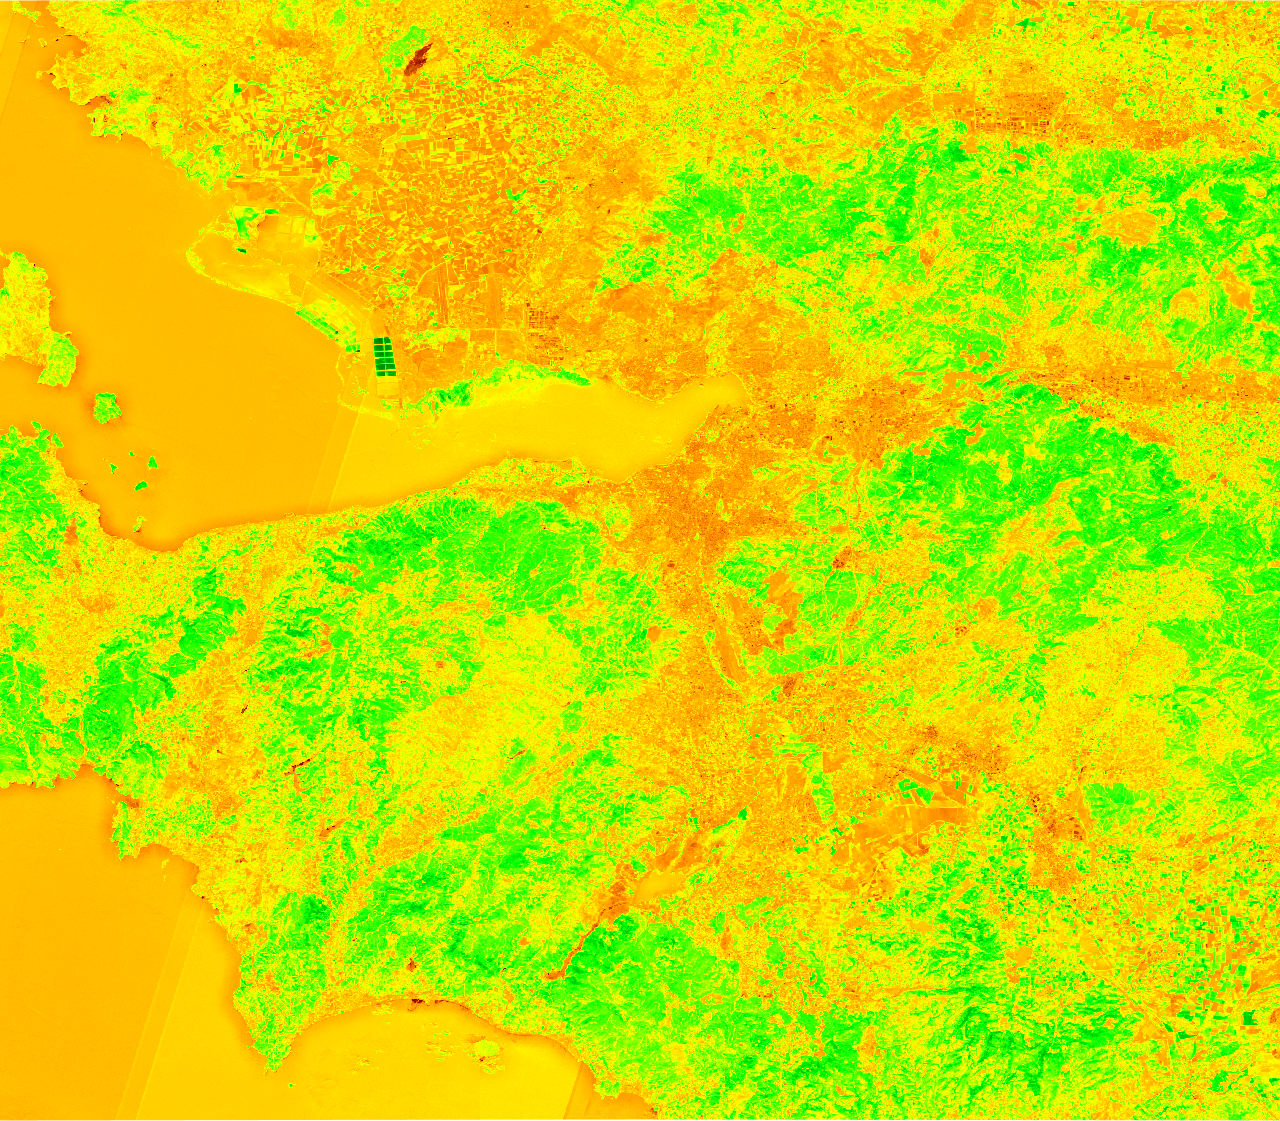
\includegraphics{../results/pre_NBR.png}}
    \caption{Pre NBR}
  \end{subfigure}\hfill
  \begin{subfigure}[b]{0.48\textwidth}
    \centering
    \resizebox{\linewidth}{!}{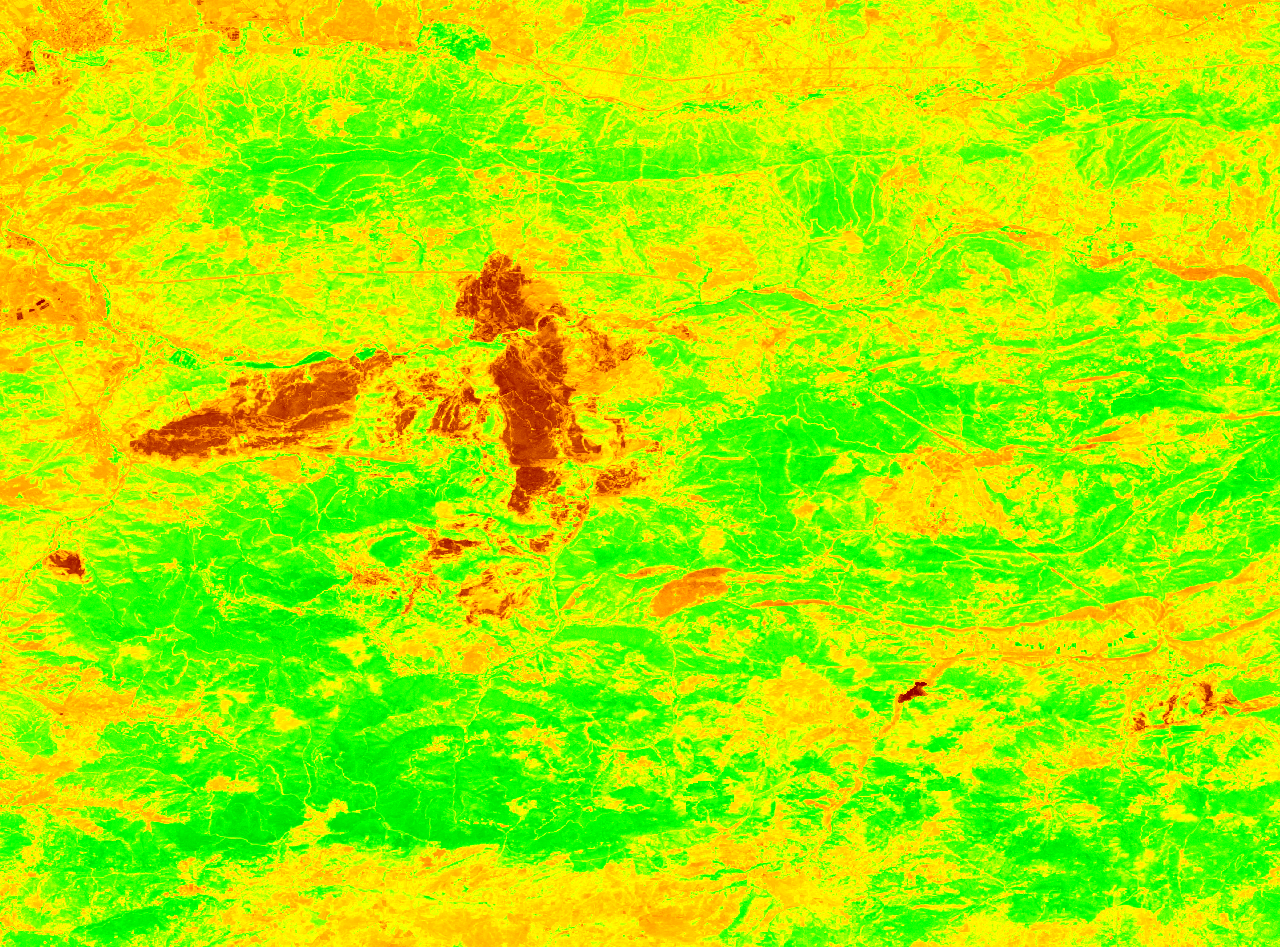
\includegraphics{../results/post_NBR.png}}
    \caption{Post NBR}
  \end{subfigure}
  \caption{NBR comparison.}
\end{figure}
\FloatBarrier

\begin{figure}[H]
  \centering
  \begin{subfigure}[b]{0.48\textwidth}
    \centering
    \resizebox{\linewidth}{!}{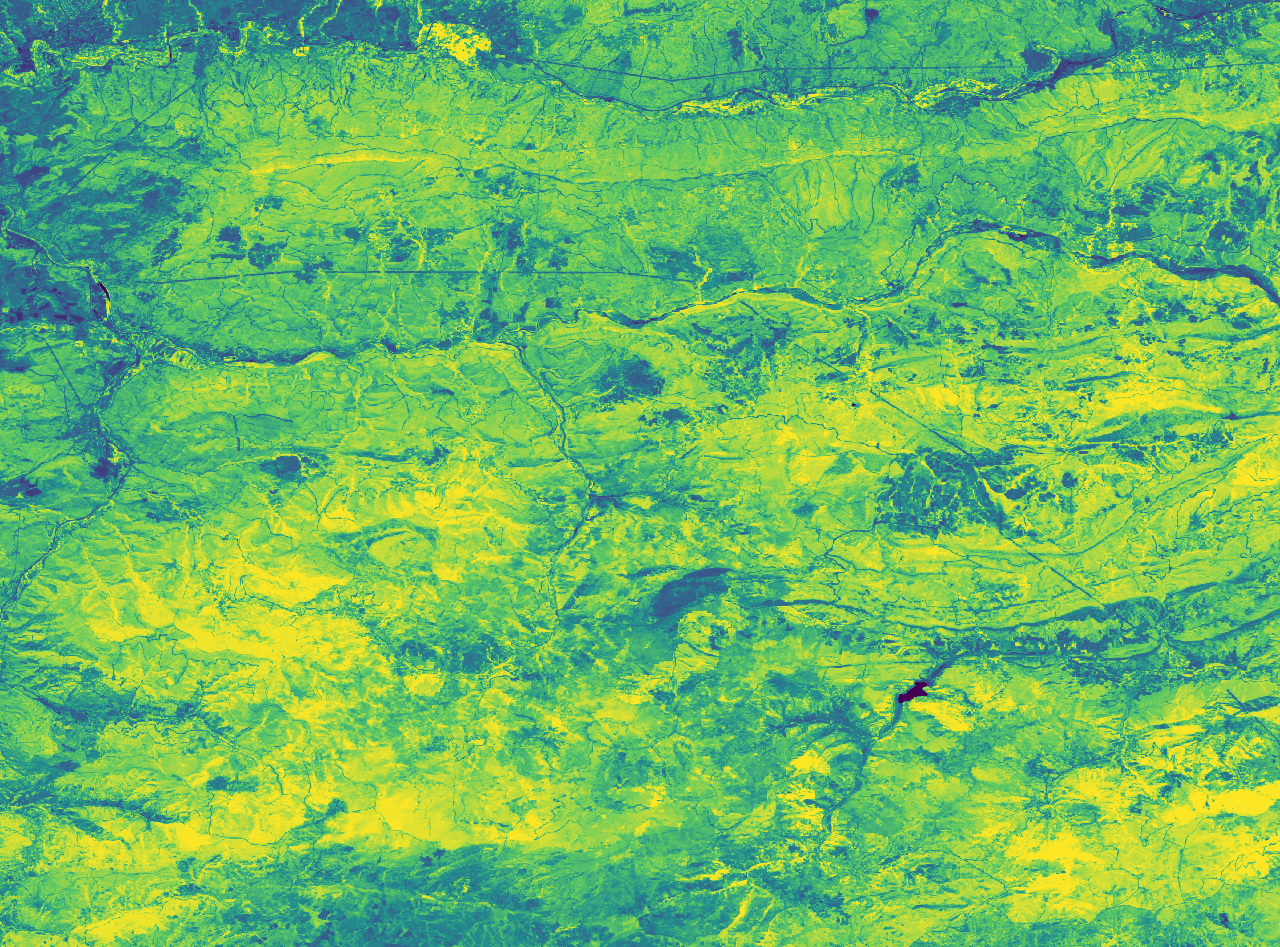
\includegraphics{../results/pre_NDVI.png}}
    \caption{Öncesi NDVI}
  \end{subfigure}\hfill
  \begin{subfigure}[b]{0.48\textwidth}
    \centering
    \resizebox{\linewidth}{!}{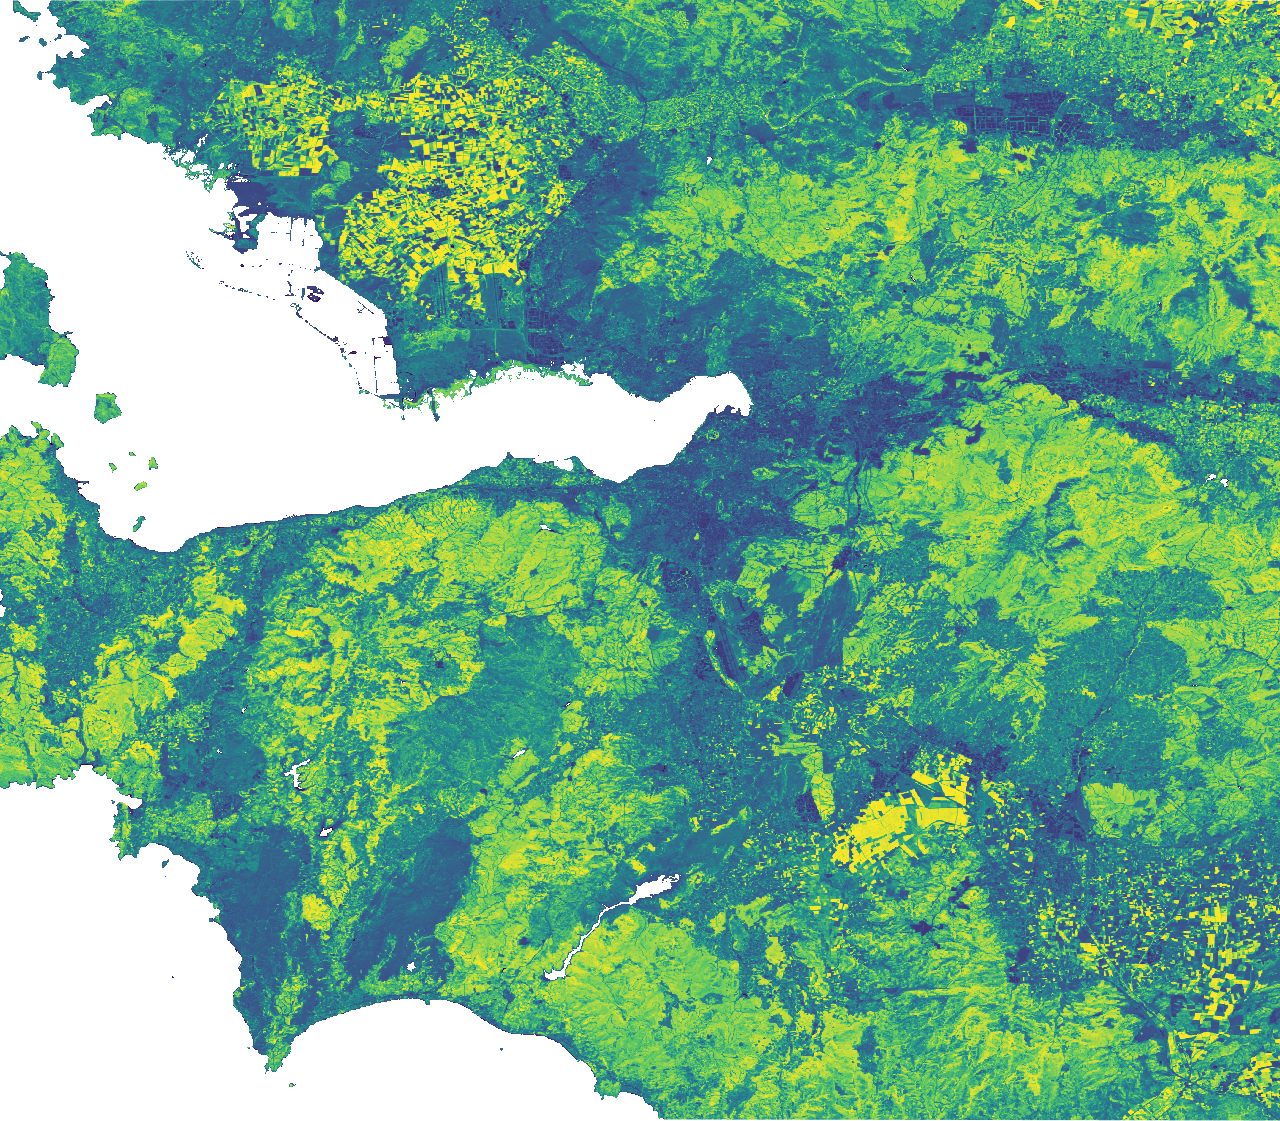
\includegraphics{../results/post_NDVI.png}}
    \caption{Sonrası NDVI}
  \end{subfigure}
  \caption{NDVI karşılaştırması.}
  \label{fig:ndvi}
\end{figure}
\FloatBarrier

\begin{figure}[H]
  \centering
  \begin{subfigure}[b]{0.48\textwidth}
    \centering
    \resizebox{\linewidth}{!}{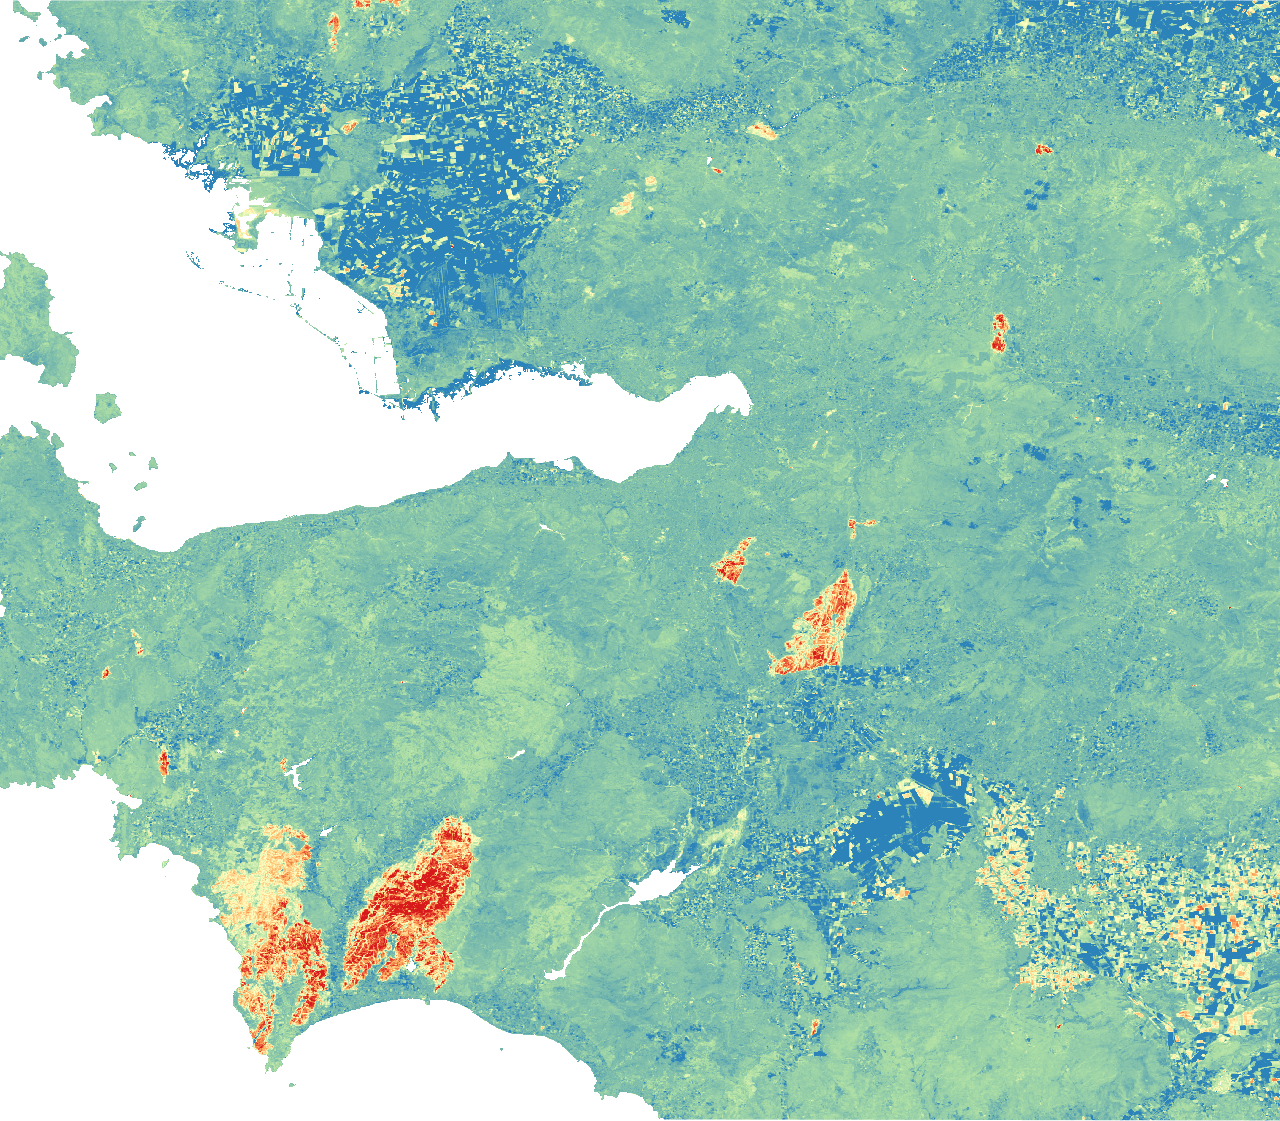
\includegraphics{../results/dNBR.png}}
    \caption{dNBR}
  \end{subfigure}\hfill
  \begin{subfigure}[b]{0.48\textwidth}
    \centering
    \resizebox{\linewidth}{!}{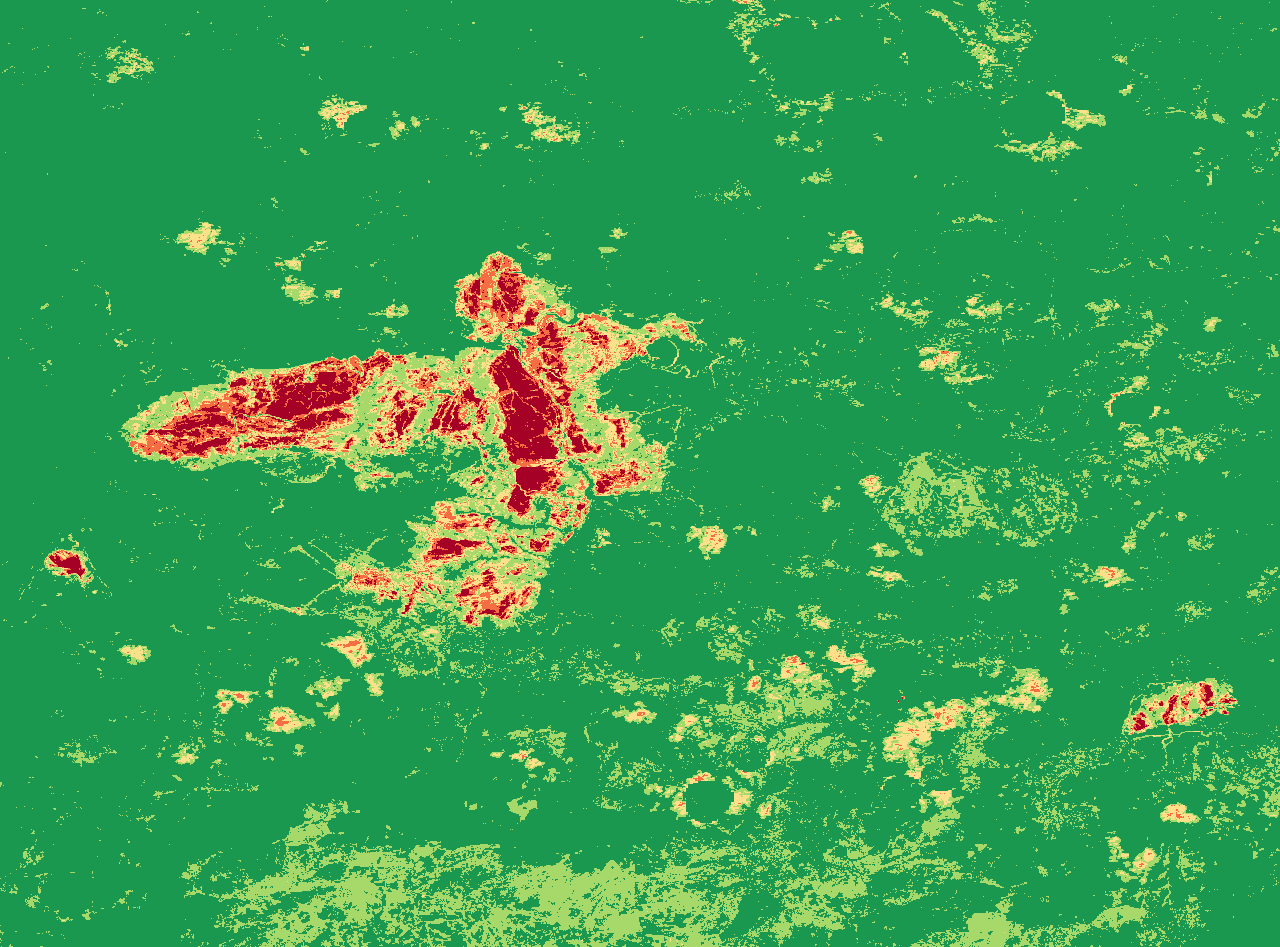
\includegraphics{../results/severity.png}}
    \caption{dNBR Şiddeti (0--4)}
  \end{subfigure}
  \caption{Fark analizi ve şiddet sınıfları.}
  \label{fig:diffs}
\end{figure}

\subsection{Özet İstatistikler}
\noindent Ortalama değerler:
\begin{itemize}
  \item \textbf{Öncesi NDVI ort.}: 0.365
  \item \textbf{Sonrası NDVI ort.}: 0.344
  \item \textbf{dNDVI ort.}: $-0.020$
  \item \textbf{dNBR ort.}: -0.038
\end{itemize}
Bu bölümde sunulan özet, yangın öncesi ve sonrası bitki örtüsü durumunu (NDVI) ve yangın etkisini (dNBR) nicel olarak ifade eder. NDVI 0 ile 1 arasında değer alır; daha yüksek değerler daha yoğun ve sağlıklı bitki örtüsünü gösterir. dNDVI iki tarih arasındaki NDVI farkıdır; negatif değerler yeşil örtüde azalmayı ifade eder. dNBR ise yanma şiddetine duyarlı bir fark ölçütüdür; yaklaşık 0.10--0.27 aralığı düşük, 0.27--0.44 aralığı orta, 0.44 ve üzeri daha yüksek şiddet seviyelerine karşılık gelir. Tablodaki ortalamalar, AOI genelinde NDVI’da \(\sim0.073\) birimlik düşüş (yaklaşık 0.584'ten 0.511'e; \(dNDVI<0\), bağıl \(\sim12.5\%\)) ve \(dNBR \approx 0.074\) ile çoğunlukla çok düşük/düşük şiddet sinyaline işaret etmektedir. Ancak bu değerler mekânsal farklılıkları düzler; yer yer daha yüksek şiddetli cepler bulunabilir. Bu nedenle yorum, şiddet haritaları ve sınıf dağılımı ile birlikte değerlendirilmelidir.

Etkilenen alan büyüklükleri, sınıf piksel sayıları ve/veya eşiklerin literatürle
karşılaştırılması ek bir tablo olarak verilebilir.

\subsection{Özet İstatistikler (CSV’den)}
Aşağıdaki tablo, analiz çıktılarından doğrudan üretilen özet değerleri göstermektedir.
\begin{table}[H]
  \centering
%  \pgfplotstabletypeset[
%     col sep=comma,
%     string type,
%     columns/metric/.style={string type,column name=Ölçüt},
%     columns/value/.style={fixed,fixed zerofill,precision=3,column name=Değer},
%     every head row/.style={before row=\toprule,after row=\midrule},
%     every last row/.style={after row=\bottomrule}
%  ]{../results/summary_stats.csv}
  \caption{Özet istatistikler (CSV'den).}
\end{table}

\subsection{Yanıklık Alanları (CSV)}
Şiddet sınıflarına göre alan dökümü (hektar cinsinden) aşağıda verilmiştir.
\begin{table}[H]
  \centering
%  \pgfplotstabletypeset[
%     col sep=comma,
%     string type,
%     columns/key/.style={string type,column name=Anahtar},
%     columns/value/.style={fixed,fixed zerofill,precision=2,column name=Alan [ha]},
%     every head row/.style={before row=\toprule,after row=\midrule},
%     every last row/.style={after row=\bottomrule}
%  ]{../results/severity_areas.csv}
  \caption{Şiddet sınıflarına göre alanlar ve toplam yanmış alan.}
\end{table}
\section{Sınırlılıklar ve Belirsizlikler}
Bulut ve duman kalıntıları, geometrik/atmosferik kalıntı hataları ve sınıflandırma
eşiklerinin genellenebilirliği sonuçları etkileyebilir. dNBR eşikleri AOI'ye ve saha
gözlemlerine göre kalibre edilmelidir. Kompozit stratejisinin (median) seçimi mekânsal
özgüllük ve bulutluluk koşullarına bağlıdır.

\section{Tartışma ve Gelecek Çalışmalar}
Yöntem, GEE altyapısıyla hızlı ve tekrarlanabilir analiz sağlar. Gelecekte RdNBR gibi
normalize edilmiş fark metriklerinin denenmesi; arazi örtüsü/sınıf bilgisi ile
birleştirilmiş analizler ve saha verisiyle karşılaştırmalı doğrulama, karar destek
perspektifinden yöntemin değerini artıracaktır. Ayrıca farklı sensörlerle (Landsat,\,Sentinel-1)
çoklu-kaynak yaklaşımı geliştirilerek zamansal kapsam ve sağlamlık genişletilebilir.

\section{Görselleştirme}
Harita görselleri, \texttt{analysis.ipynb} defterinden otomatik üretilen HTML ve PNG
çıktıları üzerinden alınmıştır. Renk paletleri ve gösterim aralıkları \texttt{src/visualize.py}
dosyasında \texttt{vis\_params()} fonksiyonunda tanımlıdır.


\end{document}














